

\hypertarget{einleitung}{%
\section{Einleitung}\label{einleitung}}

\hypertarget{motivation}{%
\subsection{Motivation}\label{motivation}}

\begin{itemize}
\tightlist
\item
  Beginn: Er zieht die Aufmerksamkeit des Lesers durch die Schilderung
  des Ereignisses auf sich, das zu dem Problem geführt hat.
\item
  Hintergrundinformationen (Herstellung des Kontexts): Gehe tiefer auf
  das Ereignis ein, indem du mehr Informationen über es vermittelst und
  dabei auch den Rahmen deiner Forschung skizzierst.
\item
  Brücke zur Problemstellung: Erläutere, inwiefern es sich hierbei um
  ein Problem handelt, und schlage somit die Brücke zur Problemstellung,
  die deiner Untersuchung zu Grunde liegt.
\end{itemize}

\hypertarget{zielsetzung}{%
\subsection{Zielsetzung}\label{zielsetzung}}

Das Ziel dieser Arbeit ist es, einen Schach-Tisch zu konstruieren und
programmieren, welcher in der Lage ist Schachfiguren autonom zu bewegen.
Der Schwerpunkt liegt dabei insbesondere auf der Programmierung des
eingebettenen Systems. Dieses besteht zum einem aus der
Positionserkennung und Steuerung der Hardwarekomponenten (Schachfiguren)
und zum anderen aus der Kommuniktation zwischen dem Tisch selbst und
einem in einer Cloud befindlichen Server.

Mittels der Programmierung werden diverse Technologien von verschiedenen
Einzelsystemen zu einem Gesamtprodukt zusammengesetzt. Zu diesen
Einzelsystemen gehören:

\begin{itemize}
\tightlist
\item
  Programmierung der Motorsteuerung, HMI (zB. Qt oder simple Buttons),
  NFC Tag erkennung
\item
  Programmierung eines Wrappers für die Kommuniktion mit der Cloud (AWS)
\item
  Statemaschiene und Implementierung der Spielflusssteuerung
\item
  Backend mit Datenbankanbindung zwischen Server und Embedded-System
\item
  Verwendung eines CI/CD Systems zum automatisierten bauen der
  Linux-Images für das Embedded-System
\end{itemize}

\hypertarget{aufbau-der-arbeit}{%
\subsection{Aufbau der Arbeit}\label{aufbau-der-arbeit}}

\begin{itemize}
\item
  theoretische Grundlagen
\item
  gegebene Randbedingungen
\item
  beleuchtung existierender ansätze \&\& festlegung zu erwartener
  Features
\item
  Kaptiel x erstellung einzelner software unf hardwarekomponenten
\item
  Kapitel x+1 zusammenführung in die DK HW
\item
  Kaptiel x+2 fehleranaöyse der DK Hardware
\item
  Kaptiel x+3 ansätze zur verbesserung und modifikation der Hardware auf
  reproduzierbarkeit und kosteneffektivität
\item
  Kaptiel x+4 test und fazit
\item
  demonstration und validierung der funktionsfähigkeit
\end{itemize}

\hypertarget{analyse-bestehender-systeme}{%
\section{Analyse bestehender
Systeme}\label{analyse-bestehender-systeme}}

\hypertarget{existierende-systeme-im-vergleich}{%
\subsection{Existierende Systeme im
Vergleich}\label{existierende-systeme-im-vergleich}}

\hypertarget{kommerzielle-produkte}{%
\subsubsection{Kommerzielle Produkte}\label{kommerzielle-produkte}}

\begin{itemize}
\tightlist
\item
  zwei hersteller wirklich autonomer schachtische; für tunieren werden
  dgt schachbretter für livestreams und recordinge verwendet.
\end{itemize}

\begin{longtable}[]{@{}lllll@{}}
\caption{Auflistung kommerzieller autonomer Schachtische}\tabularnewline
\toprule
\begin{minipage}[b]{0.18\columnwidth}\raggedright
\strut
\end{minipage} & \begin{minipage}[b]{0.18\columnwidth}\raggedright
Square Off - Kingdom \cite{squareoffkingdom}\strut
\end{minipage} & \begin{minipage}[b]{0.22\columnwidth}\raggedright
Square Off - Grand Kingdom \cite{squareoffgrand}\strut
\end{minipage} & \begin{minipage}[b]{0.15\columnwidth}\raggedright
DGT Smart Board \cite{dtgsmartboard}\strut
\end{minipage} & \begin{minipage}[b]{0.13\columnwidth}\raggedright
DGT Bluetooth Wenge \cite{dtgble}\strut
\end{minipage}\tabularnewline
\midrule
\endfirsthead
\toprule
\begin{minipage}[b]{0.18\columnwidth}\raggedright
\strut
\end{minipage} & \begin{minipage}[b]{0.18\columnwidth}\raggedright
Square Off - Kingdom \cite{squareoffkingdom}\strut
\end{minipage} & \begin{minipage}[b]{0.22\columnwidth}\raggedright
Square Off - Grand Kingdom \cite{squareoffgrand}\strut
\end{minipage} & \begin{minipage}[b]{0.15\columnwidth}\raggedright
DGT Smart Board \cite{dtgsmartboard}\strut
\end{minipage} & \begin{minipage}[b]{0.13\columnwidth}\raggedright
DGT Bluetooth Wenge \cite{dtgble}\strut
\end{minipage}\tabularnewline
\midrule
\endhead
\begin{minipage}[t]{0.18\columnwidth}\raggedright
Erkennung Schfigurstellung\strut
\end{minipage} & \begin{minipage}[t]{0.18\columnwidth}\raggedright
nein (Manuell per Ausgangsposition)\strut
\end{minipage} & \begin{minipage}[t]{0.22\columnwidth}\raggedright
nein (Manuell per Ausgangsposition)\strut
\end{minipage} & \begin{minipage}[t]{0.15\columnwidth}\raggedright
ja (Resonanzspulen)\strut
\end{minipage} & \begin{minipage}[t]{0.13\columnwidth}\raggedright
ja (\gls{rfid})\strut
\end{minipage}\tabularnewline
\begin{minipage}[t]{0.18\columnwidth}\raggedright
Tischabmessungen (LxBxH)\strut
\end{minipage} & \begin{minipage}[t]{0.18\columnwidth}\raggedright
486mm x 486mm x 75mm\strut
\end{minipage} & \begin{minipage}[t]{0.22\columnwidth}\raggedright
671mm x 486mm x 75mm\strut
\end{minipage} & \begin{minipage}[t]{0.15\columnwidth}\raggedright
540mm x 540mm x 20mm\strut
\end{minipage} & \begin{minipage}[t]{0.13\columnwidth}\raggedright
540mm x 540mm x 20mm\strut
\end{minipage}\tabularnewline
\begin{minipage}[t]{0.18\columnwidth}\raggedright
Konnektivität\strut
\end{minipage} & \begin{minipage}[t]{0.18\columnwidth}\raggedright
\gls{ble}\strut
\end{minipage} & \begin{minipage}[t]{0.22\columnwidth}\raggedright
\gls{ble}\strut
\end{minipage} & \begin{minipage}[t]{0.15\columnwidth}\raggedright
\gls{usb} / Seriell\strut
\end{minipage} & \begin{minipage}[t]{0.13\columnwidth}\raggedright
Bluetooth 2.0\strut
\end{minipage}\tabularnewline
\begin{minipage}[t]{0.18\columnwidth}\raggedright
Automatisches Bewegen der Figuren\strut
\end{minipage} & \begin{minipage}[t]{0.18\columnwidth}\raggedright
ja\strut
\end{minipage} & \begin{minipage}[t]{0.22\columnwidth}\raggedright
ja\strut
\end{minipage} & \begin{minipage}[t]{0.15\columnwidth}\raggedright
nein\strut
\end{minipage} & \begin{minipage}[t]{0.13\columnwidth}\raggedright
nein\strut
\end{minipage}\tabularnewline
\begin{minipage}[t]{0.18\columnwidth}\raggedright
Spiel Livestream\strut
\end{minipage} & \begin{minipage}[t]{0.18\columnwidth}\raggedright
ja\strut
\end{minipage} & \begin{minipage}[t]{0.22\columnwidth}\raggedright
ja\strut
\end{minipage} & \begin{minipage}[t]{0.15\columnwidth}\raggedright
ja\strut
\end{minipage} & \begin{minipage}[t]{0.13\columnwidth}\raggedright
ja\strut
\end{minipage}\tabularnewline
\begin{minipage}[t]{0.18\columnwidth}\raggedright
Cloud anbindung (online Spiele)\strut
\end{minipage} & \begin{minipage}[t]{0.18\columnwidth}\raggedright
ja (über Mobiltelefon + App)\strut
\end{minipage} & \begin{minipage}[t]{0.22\columnwidth}\raggedright
ja (über Mobiltelefon + App)\strut
\end{minipage} & \begin{minipage}[t]{0.15\columnwidth}\raggedright
ja (über PC + App)\strut
\end{minipage} & \begin{minipage}[t]{0.13\columnwidth}\raggedright
ja (über PC + App)\strut
\end{minipage}\tabularnewline
\begin{minipage}[t]{0.18\columnwidth}\raggedright
Parkposition für ausgeschiedene Figuren\strut
\end{minipage} & \begin{minipage}[t]{0.18\columnwidth}\raggedright
nein\strut
\end{minipage} & \begin{minipage}[t]{0.22\columnwidth}\raggedright
ja\strut
\end{minipage} & \begin{minipage}[t]{0.15\columnwidth}\raggedright
nein\strut
\end{minipage} & \begin{minipage}[t]{0.13\columnwidth}\raggedright
nein\strut
\end{minipage}\tabularnewline
\begin{minipage}[t]{0.18\columnwidth}\raggedright
Stand-Alone Funktionalität\strut
\end{minipage} & \begin{minipage}[t]{0.18\columnwidth}\raggedright
nein (Mobiltelefon erforderlich)\strut
\end{minipage} & \begin{minipage}[t]{0.22\columnwidth}\raggedright
nein (Mobiltelefon erforderlich)\strut
\end{minipage} & \begin{minipage}[t]{0.15\columnwidth}\raggedright
nein (PC erforderlich)\strut
\end{minipage} & \begin{minipage}[t]{0.13\columnwidth}\raggedright
nein (PC erforderlich)\strut
\end{minipage}\tabularnewline
\begin{minipage}[t]{0.18\columnwidth}\raggedright
Besonderheiten\strut
\end{minipage} & \begin{minipage}[t]{0.18\columnwidth}\raggedright
Akku für 30 Spiele\strut
\end{minipage} & \begin{minipage}[t]{0.22\columnwidth}\raggedright
Akku für 15 Spiele\strut
\end{minipage} & \begin{minipage}[t]{0.15\columnwidth}\raggedright
-\strut
\end{minipage} & \begin{minipage}[t]{0.13\columnwidth}\raggedright
-\strut
\end{minipage}\tabularnewline
\bottomrule
\end{longtable}

\hypertarget{open-source-projekte}{%
\subsubsection{Open-Source Projekte}\label{open-source-projekte}}

Bei allen Open-Source Projekten wurden die Features anhand der
Beschreibung und der aktuellen Software extrahiert. Besonders bei
work-in-progress Projekten können sich die Features noch verändern und
so weitere Funktionalitäten hinzugefügt werden.

Desweiteren gibt es unzählige deratige Projekte, in der Tabelle wurde
nur diese Aufgelistet welche sich von anderen Projekten in mindestens
einem Feature unterscheiden.

Auch existieren weitere abwandlungen von autonomen Schachbrettern, bei
welchem die Figuren von oberhalb des Spielbretts gegriffen bzw bewegt
werden. In einigen Projekten wird dies mittels eines Roboterarms
\cite{actprojectrobot} oder eines modifizierten 3D-Druckers
realisiert, diese wurden hier nicht berücksichtigt.

\begin{longtable}[]{@{}llll@{}}
\caption{Auflistung von Open-Source Schachtisch
Projekten}\tabularnewline
\toprule
\begin{minipage}[b]{0.24\columnwidth}\raggedright
\strut
\end{minipage} & \begin{minipage}[b]{0.24\columnwidth}\raggedright
Automated Chess Board (Michael Guerero)\strut
\end{minipage} & \begin{minipage}[b]{0.25\columnwidth}\raggedright
Automated Chess Board (Akash Ravichandran)\strut
\end{minipage} & \begin{minipage}[b]{0.16\columnwidth}\raggedright
DIY Super Smart Chessboard\strut
\end{minipage}\tabularnewline
\midrule
\endfirsthead
\toprule
\begin{minipage}[b]{0.24\columnwidth}\raggedright
\strut
\end{minipage} & \begin{minipage}[b]{0.24\columnwidth}\raggedright
Automated Chess Board (Michael Guerero)\strut
\end{minipage} & \begin{minipage}[b]{0.25\columnwidth}\raggedright
Automated Chess Board (Akash Ravichandran)\strut
\end{minipage} & \begin{minipage}[b]{0.16\columnwidth}\raggedright
DIY Super Smart Chessboard\strut
\end{minipage}\tabularnewline
\midrule
\endhead
\begin{minipage}[t]{0.24\columnwidth}\raggedright
Erkennung Schfigurstellung\strut
\end{minipage} & \begin{minipage}[t]{0.24\columnwidth}\raggedright
nein (Manuell per Ausgangsposition)\strut
\end{minipage} & \begin{minipage}[t]{0.25\columnwidth}\raggedright
ja (Kamera / OpenCV)\strut
\end{minipage} & \begin{minipage}[t]{0.16\columnwidth}\raggedright
nein\strut
\end{minipage}\tabularnewline
\begin{minipage}[t]{0.24\columnwidth}\raggedright
Tischabmessungen (LxBxH)\strut
\end{minipage} & \begin{minipage}[t]{0.24\columnwidth}\raggedright
keine Angabe\strut
\end{minipage} & \begin{minipage}[t]{0.25\columnwidth}\raggedright
keine Angabe\strut
\end{minipage} & \begin{minipage}[t]{0.16\columnwidth}\raggedright
450mm x 300mm x 50mm\strut
\end{minipage}\tabularnewline
\begin{minipage}[t]{0.24\columnwidth}\raggedright
Konnektivität\strut
\end{minipage} & \begin{minipage}[t]{0.24\columnwidth}\raggedright
\gls{usb}\strut
\end{minipage} & \begin{minipage}[t]{0.25\columnwidth}\raggedright
Ethernet\strut
\end{minipage} & \begin{minipage}[t]{0.16\columnwidth}\raggedright
\gls{wlan}\strut
\end{minipage}\tabularnewline
\begin{minipage}[t]{0.24\columnwidth}\raggedright
Automatisches Bewegen der Figuren\strut
\end{minipage} & \begin{minipage}[t]{0.24\columnwidth}\raggedright
ja\strut
\end{minipage} & \begin{minipage}[t]{0.25\columnwidth}\raggedright
ja\strut
\end{minipage} & \begin{minipage}[t]{0.16\columnwidth}\raggedright
nein\strut
\end{minipage}\tabularnewline
\begin{minipage}[t]{0.24\columnwidth}\raggedright
Spiel Livestream\strut
\end{minipage} & \begin{minipage}[t]{0.24\columnwidth}\raggedright
nein\strut
\end{minipage} & \begin{minipage}[t]{0.25\columnwidth}\raggedright
nein\strut
\end{minipage} & \begin{minipage}[t]{0.16\columnwidth}\raggedright
nein\strut
\end{minipage}\tabularnewline
\begin{minipage}[t]{0.24\columnwidth}\raggedright
Cloud anbindung (online Spiele)\strut
\end{minipage} & \begin{minipage}[t]{0.24\columnwidth}\raggedright
nein\strut
\end{minipage} & \begin{minipage}[t]{0.25\columnwidth}\raggedright
nein\strut
\end{minipage} & \begin{minipage}[t]{0.16\columnwidth}\raggedright
ja\strut
\end{minipage}\tabularnewline
\begin{minipage}[t]{0.24\columnwidth}\raggedright
Parkposition für ausgeschiedene Figuren\strut
\end{minipage} & \begin{minipage}[t]{0.24\columnwidth}\raggedright
nein\strut
\end{minipage} & \begin{minipage}[t]{0.25\columnwidth}\raggedright
nein\strut
\end{minipage} & \begin{minipage}[t]{0.16\columnwidth}\raggedright
nein\strut
\end{minipage}\tabularnewline
\begin{minipage}[t]{0.24\columnwidth}\raggedright
Stand-Alone Funktionalität\strut
\end{minipage} & \begin{minipage}[t]{0.24\columnwidth}\raggedright
nein (PC erfoderlich)\strut
\end{minipage} & \begin{minipage}[t]{0.25\columnwidth}\raggedright
ja\strut
\end{minipage} & \begin{minipage}[t]{0.16\columnwidth}\raggedright
ja\strut
\end{minipage}\tabularnewline
\begin{minipage}[t]{0.24\columnwidth}\raggedright
Besonderheiten\strut
\end{minipage} & \begin{minipage}[t]{0.24\columnwidth}\raggedright
-\strut
\end{minipage} & \begin{minipage}[t]{0.25\columnwidth}\raggedright
Sprachsteuerung (Amazon Alexa)\strut
\end{minipage} & \begin{minipage}[t]{0.16\columnwidth}\raggedright
Zuganzeige über LED Matrix\strut
\end{minipage}\tabularnewline
\begin{minipage}[t]{0.24\columnwidth}\raggedright
Licence\strut
\end{minipage} & \begin{minipage}[t]{0.24\columnwidth}\raggedright
\gls{gpl} 3+\strut
\end{minipage} & \begin{minipage}[t]{0.25\columnwidth}\raggedright
\gls{gpl}\strut
\end{minipage} & \begin{minipage}[t]{0.16\columnwidth}\raggedright
-\strut
\end{minipage}\tabularnewline
\bottomrule
\end{longtable}

\hypertarget{zielgruppe}{%
\subsection{Zielgruppe}\label{zielgruppe}}

\hypertarget{user-experience}{%
\subsection{User Experience}\label{user-experience}}

\hypertarget{software-aufbau}{%
\subsubsection{Software-Aufbau}\label{software-aufbau}}

\hypertarget{hardware-aufbau}{%
\subsubsection{Hardware-Aufbau}\label{hardware-aufbau}}

\hypertarget{grundlagen}{%
\section{Grundlagen}\label{grundlagen}}

\hypertarget{anforderungsanalyse}{%
\subsection{Anforderungsanalyse}\label{anforderungsanalyse}}

\hypertarget{machbarkeitsanalyse}{%
\subsection{Machbarkeitsanalyse}\label{machbarkeitsanalyse}}

\hypertarget{technologien-im-makerspace}{%
\subsection{Technologien im
Makerspace}\label{technologien-im-makerspace}}

\hypertarget{section}{%
\subsection{}\label{section}}

\hypertarget{vinaque-sanguine-metuenti-cuiquam-alcyone-fixus}{%
\section{Vinaque sanguine metuenti cuiquam Alcyone
fixus}\label{vinaque-sanguine-metuenti-cuiquam-alcyone-fixus}}

\hypertarget{aesculeae-domus-vincemur-et-veneris-adsuetus-lapsum}{%
\subsection{Aesculeae domus vincemur et Veneris adsuetus
lapsum}\label{aesculeae-domus-vincemur-et-veneris-adsuetus-lapsum}}

Lorem markdownum Letoia, et alios: figurae flectentem annis aliquid
Peneosque ab esse, obstat gravitate. Obscura atque coniuge, per de
coniunx, sibi \textbf{medias commentaque virgine} anima tamen comitemque
petis, sed. In Amphion vestros hamos ire arceor mandere spicula, in
licet aliquando.

\begin{lstlisting}[language=Java]
public class Example implements LoremIpsum {
    public static void main(String[] args) {
        if(args.length < 2) {
            System.out.println("Lorem ipsum dolor sit amet");
        }
    } // Obscura atque coniuge, per de coniunx
}
\end{lstlisting}

Listing: TEST

\begin{lstlisting}[language={C++}]
// Your First C++ Program

#include <iostream>

int main() {
    std::cout << "Hello World!";
    return 0;
}

}
\end{lstlisting}

Porrigitur et Pallas nuper longusque cratere habuisse sepulcro pectore
fertur. Laudat ille auditi; vertitur iura tum nepotis causa; motus. Diva
virtus! Acrota destruitis vos iubet quo et classis excessere Scyrumve
spiro subitusque mente Pirithoi abstulit, lapides.

\hypertarget{lydia-caelo-recenti-haerebat-lacerum-ratae-at}{%
\subsection{Lydia caelo recenti haerebat lacerum ratae
at}\label{lydia-caelo-recenti-haerebat-lacerum-ratae-at}}

Te concepit pollice fugit vias alumno \textbf{oras} quam potest
\href{http://example.com\#rursus}{rursus} optat. Non evadere orbem
equorum, spatiis, vel pede inter si.

\begin{enumerate}
\def\labelenumi{\arabic{enumi}.}
\tightlist
\item
  De neque iura aquis
\item
  Frangitur gaudia mihi eo umor terrae quos
\item
  Recens diffudit ille tantum
\end{enumerate}

\begin{equation}\label{eq:neighbor-propability}
    p_{ij}(t) = \frac{\ell_j(t) - \ell_i(t)}{\sum_{k \in N_i(t)}^{} \ell_k(t) - \ell_i(t)}
\end{equation}

Tamen condeturque saxa Pallorque num et ferarum promittis inveni lilia
iuvencae adessent arbor. Florente perque at condeturque saxa et ferarum
promittis tendebat. Armos nisi obortas refugit me.

\begin{quote}
Et nepotes poterat, se qui. Euntem ego pater desuetaque aethera
Maeandri, et \href{http://example.com\#Dardanio_geminaque}{Dardanio
geminaque} cernit. Lassaque poenas nec, manifesta \(\pi r^2\) mirantia
captivarum prohibebant scelerato gradus unusque dura.
\end{quote}

\begin{itemize}
\tightlist
\item
  Permulcens flebile simul
\item
  Iura tum nepotis causa motus diva virtus Acrota. Tamen condeturque
  saxa Pallorque num et ferarum promittis inveni lilia iuvencae adessent
  arbor. Florente perque at ire arcum.
\end{itemize}

\hypertarget{image-with-caption}{%
\subsection{Image with Caption}\label{image-with-caption}}

\begin{figure}
\centering
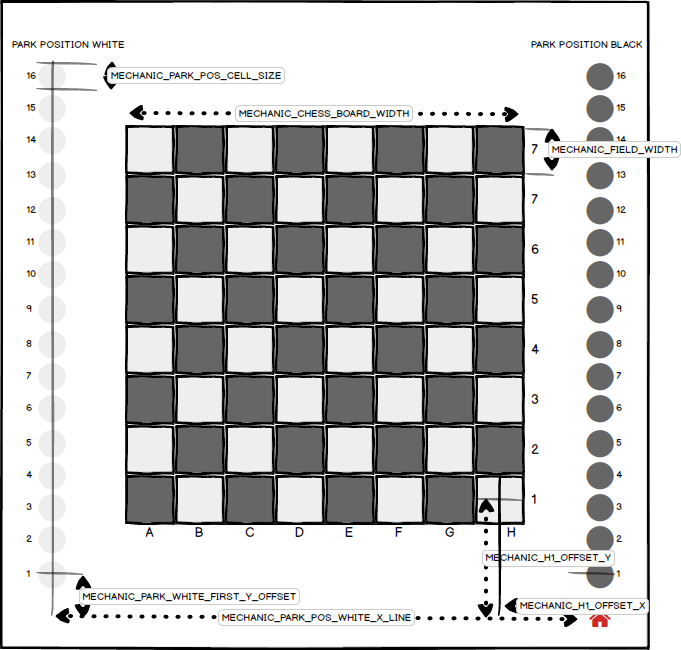
\includegraphics{images/ATC_Calibration_Guide.png}
\caption{Kalibrierungeschema der Mechanik zeigt welche Abstände in der
Konfiguration eigetragen werden müssen}
\end{figure}